\documentclass{article}
\usepackage{caption}
\usepackage{subcaption}
\usepackage{graphicx}
\usepackage{tikz}
\usepackage{tikzsymbols}
\usetikzlibrary{calc}
\usepackage{float}
\usepackage{pdflscape}
\usepackage{geometry}
\geometry{a4paper, landscape, margin=1cm}
\pagestyle{empty}

\def\centerarc[#1](#2)(#3:#4:#5){\draw[#1] ($(#2)+({#5*cos(#3)},{#5*sin(#3)})$) arc (#3:#4:#5);}

\begin{document}
	\centering
	\begin{figure}[H]
			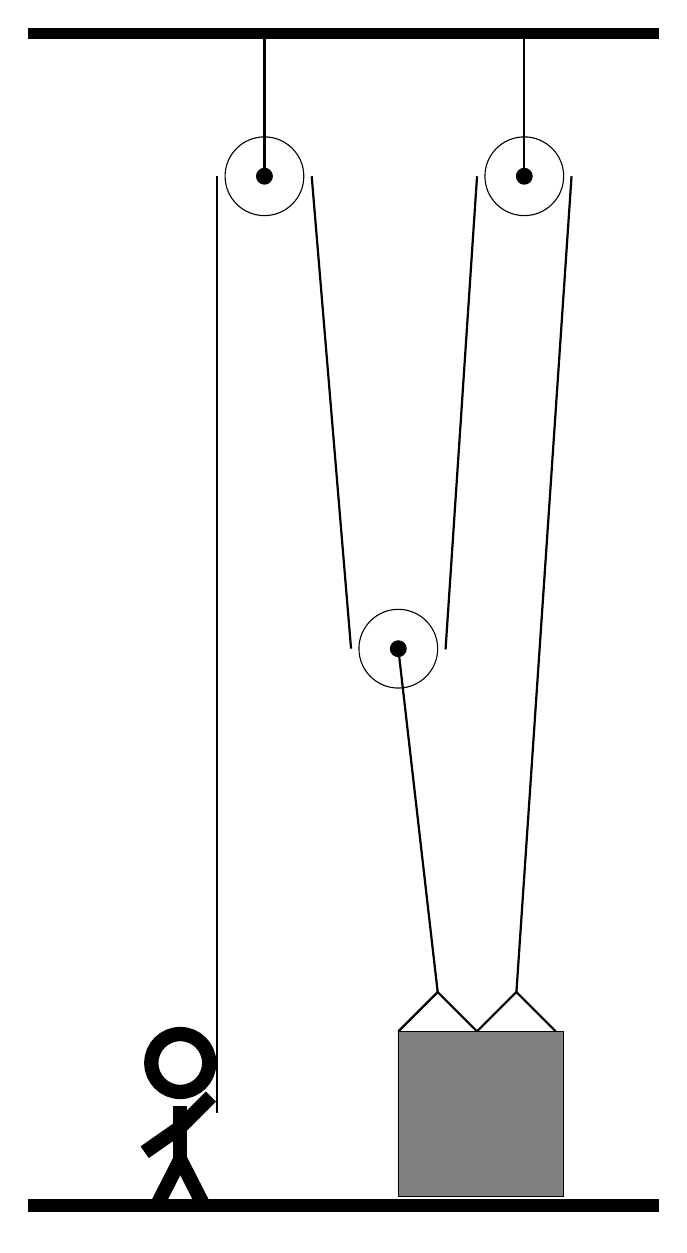
\begin{tikzpicture}
				%%%%% START %%%%%
								
				\draw[fill=black] (-2, 11.75) rectangle (6, 11.88);
				
				\draw (1, 10) circle (0.5);
				\draw[fill=black] (1, 10) circle (0.1);
				\draw[thick] (1, 10) -- (1, 11.75);
				
				\draw (4.3, 10) circle (0.5);
				\draw[fill=black] (4.3, 10) circle (0.1);
				\draw[thick] (4.3, 10) -- (4.3, 11.75);
				
				\draw (2.7, 4) circle (0.5);
				\draw[fill=black] (2.7, 4) circle (0.1);
				
				
				\draw[thick]  (2.7, -0.86) -- (3.2, -0.36) -- (3.7, -0.86);
				\draw[thick]  (3.7, -0.86) -- (4.2, -0.36) -- (4.7, -0.86);
				\draw[fill=black!50] (2.7, -0.86) rectangle (4.8, -2.96);
				
				\draw[thick] (0.4, -1.9) -- (0.4, 10);
				\centerarc[thick](1, 10)(0:180:0.6);
				\draw[thick] (1.6, 10) -- (2.1, 4);
				\centerarc[thick](2.7, 4)(180:370:0.6);
				\draw[thick] (3.3, 3.99) -- (3.7, 10);
				\centerarc[thick](4.3, 10)(0:180:0.6);
				\draw[thick] (4.2, -0.36) -- (4.9, 10);
				\draw[thick] (3.2, -0.36) -- (2.7, 4);
				
				\node at (-0.1, -2) {\Strichmaxerl[10][35][45]};
				
				\draw[fill=black] (-2, -3) rectangle (6, -3.15);
				%%%%% END %%%%%
			\end{tikzpicture}
	\end{figure}	
\end{document}